\section{Phân tích và Đặc tả Yêu cầu Hệ thống}

\subsection{Xác định các Tác nhân (Actors)}
Dựa trên mô hình kinh doanh nền tảng đa lăng kính (Multi-sided Platform) kết hợp SaaS, hệ thống CourtMate phục vụ ba nhóm tác nhân chính:
\begin{itemize}
    \item \textbf{Người chơi (B2C Customer):} Những cá nhân có nhu cầu tìm kiếm sân thể thao (Pickleball, Cầu lông, Tennis), mong muốn đặt lịch nhanh chóng, tiện lợi và thanh toán trực tuyến.
    \item \textbf{Chủ sân (B2B Partner):} Các đối tác sở hữu cụm sân, cần một hệ thống quản lý lịch trình, cơ sở vật chất, chống thất thoát doanh thu và tối ưu hóa công suất khai thác sân thông qua cấu hình giá động.
    \item \textbf{Quản trị viên hệ thống (System Admin):} Đội ngũ vận hành nền tảng CourtMate, chịu trách nhiệm quản lý tài khoản đối tác, theo dõi dòng tiền và giám sát hoạt động kỹ thuật của hệ thống.
\end{itemize}

\subsection{Biểu đồ Use Case tổng quát}
Biểu đồ Use Case tổng quát thể hiện bức tranh toàn cảnh về cách thức các tác nhân tương tác với hệ thống CourtMate, đảm bảo sự phân tách rõ ràng giữa luồng nghiệp vụ B2C (đặt sân) và B2B (quản lý, vận hành).

\begin{figure}[H]
    \centering
    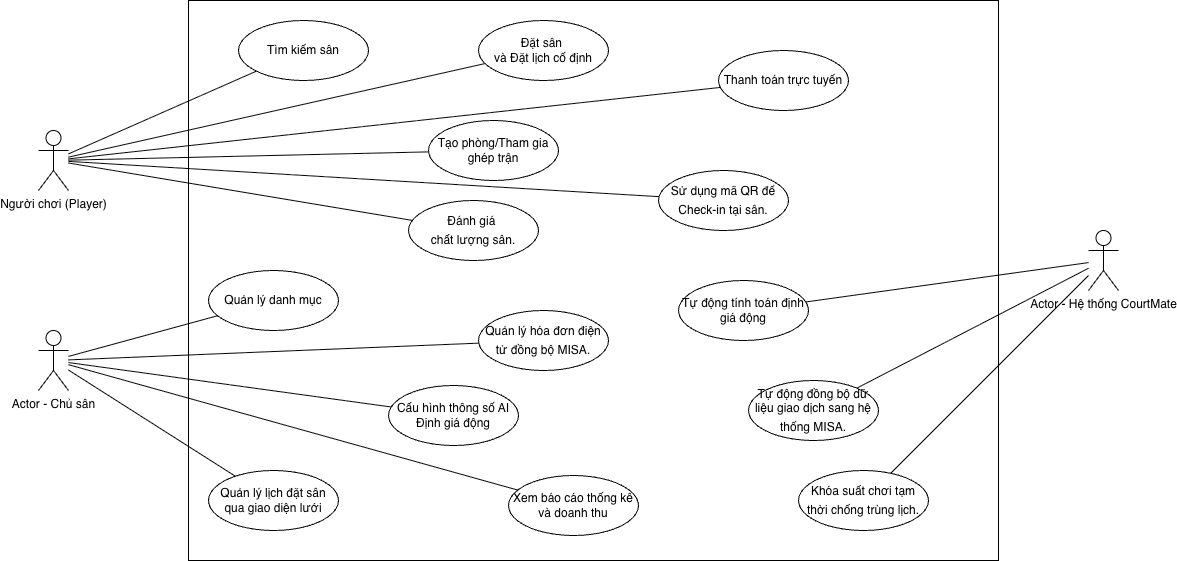
\includegraphics[width=0.95\textwidth]{Images/TMĐT_252-use_case.drawio.png}
    \caption{Biểu đồ Use Case tổng quát của hệ thống CourtMate}
    \label{fig:general_usecase}
\end{figure}

\subsection{Danh sách các Use Case chính}
Hệ thống cung cấp các nhóm chức năng cốt lõi được phân chia theo từng nhóm tác nhân cụ thể. Chi tiết các Use Case được trình bày trong bảng dưới đây:

\begin{table}[H]
    \centering
    \renewcommand{\arraystretch}{1.4}
    \begin{tabular}{|p{4.5cm}|p{3cm}|p{7.5cm}|}
        \hline
        \textbf{Tên Use Case} & \textbf{Tác nhân chính} & \textbf{Mô tả tóm tắt} \\
        \hline
        \multicolumn{3}{|c|}{\textbf{Nhóm: Dành cho Người chơi}} \\
        \hline
        Tìm kiếm sân & Người chơi & Tìm sân theo vị trí, bản đồ không gian và tiện ích. \\
        \hline
        Đặt sân và Đặt lịch cố định & Người chơi & Chọn khung giờ trống để đặt lẻ hoặc đặt cố định định kỳ. \\
        \hline
        Thanh toán trực tuyến & Người chơi & Thực hiện thanh toán khép kín qua MoMo, ZaloPay, VietQR. \\
        \hline
        Tạo phòng/Tham gia ghép trận & Người chơi & Hệ thống Matchmaking giúp người chơi tìm đồng đội cùng trình độ. \\
        \hline
        Check-in tại sân bằng mã QR & Người chơi & Quét mã tại quầy để xác nhận sự hiện diện (Check-in). \\
        \hline
        Đánh giá chất lượng sân & Người chơi & Viết review và chấm điểm sân sau khi hoàn thành buổi chơi. \\
        \hline
        \multicolumn{3}{|c|}{\textbf{Nhóm: Dành cho Chủ sân}} \\
        \hline
        Quản lý danh mục & Chủ sân & Thêm, sửa, xóa thông tin cụm sân (Venue) và các sân lẻ (Court). \\
        \hline
        Quản lý lịch đặt sân & Chủ sân & Kéo-thả trực quan để tạo/dời lịch, nắm bắt trạng thái sân realtime. \\
        \hline
        Cấu hình AI Định giá động & Chủ sân & Thiết lập biên độ giảm/tăng giá, trọng số thời tiết cho AI. \\
        \hline
        Quản lý hóa đơn điện tử & Chủ sân & Quản lý và đối soát các hóa đơn điện tử đã được tự động sinh ra. \\
        \hline
        Xem báo cáo thống kê & Chủ sân & Xem biểu đồ nhiệt (Heatmap), báo cáo tài chính và công suất. \\
        \hline
        \multicolumn{3}{|c|}{\textbf{Nhóm: Hệ thống tự động}} \\
        \hline
        Tính toán định giá động & Hệ thống & AI tự động phân tích dữ liệu và cập nhật hệ số giá (Multiplier). \\
        \hline
        Đồng bộ giao dịch sang MISA & Hệ thống & Gọi API sang MISA xuất hóa đơn ngay sau khi thanh toán. \\
        \hline
        Khóa suất chơi tạm thời & Hệ thống & Cơ chế Optimistic Lock giữ chỗ tạm thời khi khách thanh toán. \\
        \hline
    \end{tabular}
    \caption{Danh sách các Use Case chính của hệ thống CourtMate}
    \label{tab:usecase_list}
\end{table}

\subsection{Đặc tả Use Case trọng tâm: Đặt sân và Thanh toán (B2C)}
\textbf{Tác nhân:} Người chơi \\
\textbf{Mục đích:} Cho phép người chơi tìm kiếm sân trống phù hợp, đặt chỗ và thanh toán trực tuyến trong một luồng duy nhất (Single-page flow).\\
\textbf{Luồng sự kiện chính:}
\begin{enumerate}
    \item Người chơi sử dụng thanh tìm kiếm và bộ lọc để tìm sân trống theo môn thể thao, vị trí, ngày và giờ.
    \item Hệ thống hiển thị danh sách các sân thỏa mãn điều kiện và bản đồ tương tác.
    \item Người chơi chọn một sân và khung giờ cụ thể.
    \item Hệ thống tự động khóa slot (Locking Slot) trong 10 phút để tránh trùng lịch (Race Condition).
    \item Người chơi chọn các dịch vụ đi kèm (nếu có) và tiến hành thanh toán bằng mã QR/Ví điện tử.
    \item Hệ thống nhận Webhook thanh toán thành công, cập nhật trạng thái đơn đặt sân thành "Đã xác nhận".
    \item Hệ thống gửi thông báo xác nhận đến Người chơi và cập nhật ngay lập tức lên Lưới lịch của Chủ sân.
\end{enumerate}

\begin{figure}[H]
    \centering
    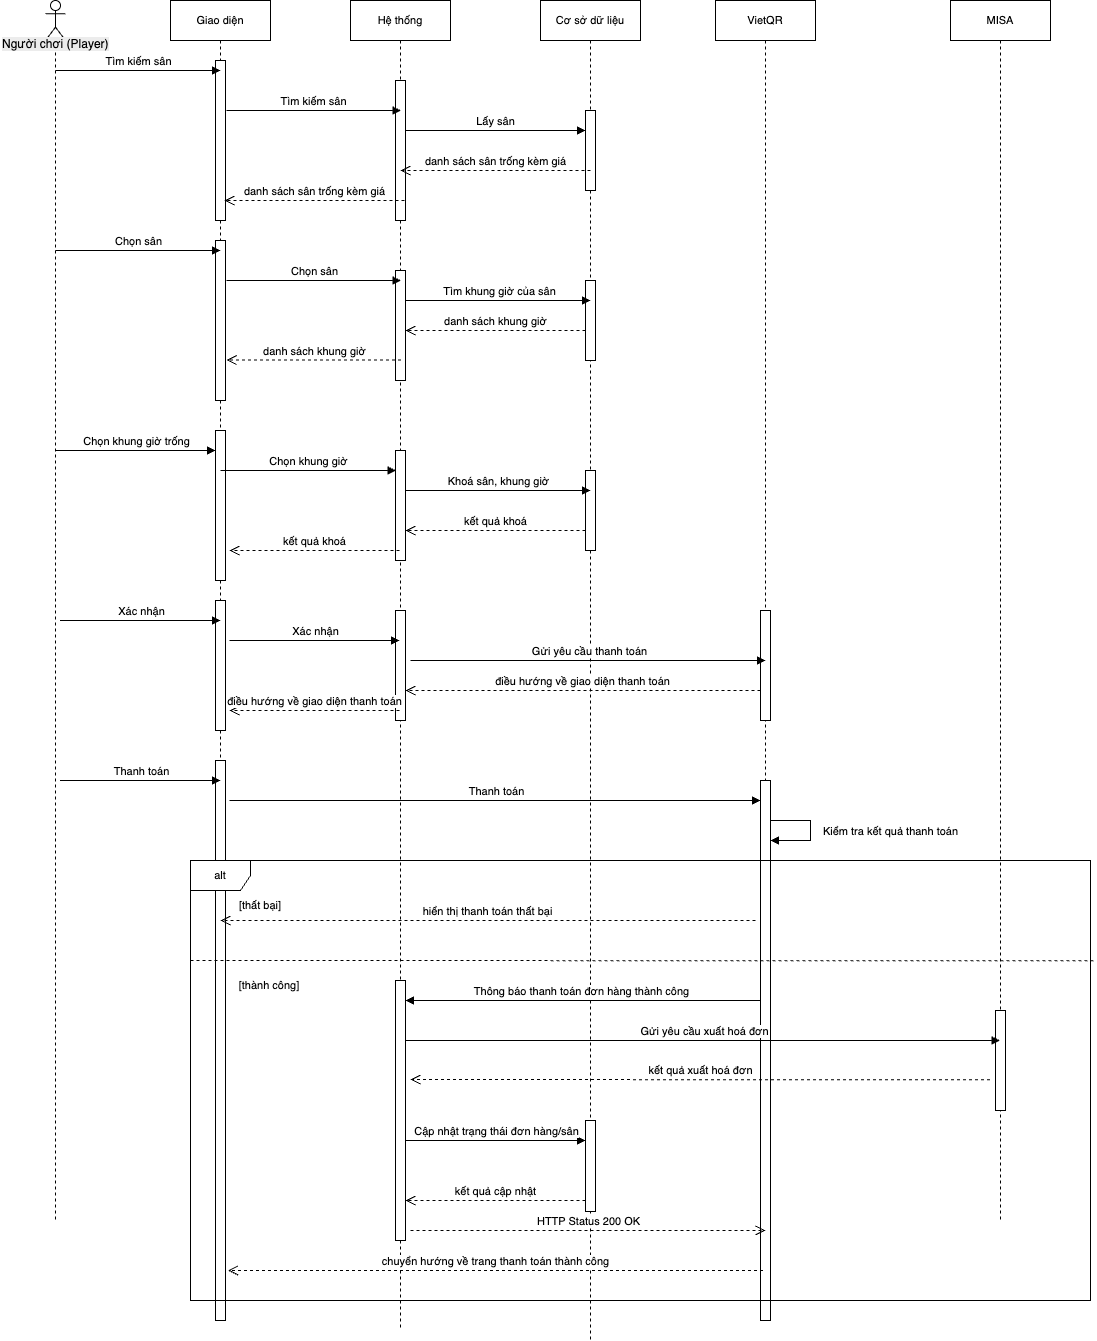
\includegraphics[width=0.95\textwidth]{Images/sq_dat_san_va_thanh_toan.png}
    \caption{Biểu đồ tuần tự (Sequence Diagram) luồng Đặt sân và Thanh toán}
    \label{fig:sequence_booking}
\end{figure}

\subsection{Đặc tả Use Case: Quản lý lưới lịch (Slot Grid) và Định giá}
\textbf{Tác nhân:} Chủ sân \\
\textbf{Mục đích:} Cung cấp công cụ quản trị trực quan để theo dõi, điều chỉnh lịch đặt sân và xử lý các tình huống phát sinh tại sân.\\
\textbf{Luồng sự kiện chính:}
\begin{enumerate}
    \item Chủ sân đăng nhập vào Smart Admin Panel (B2B).
    \item Hệ thống truy xuất dữ liệu và hiển thị Lưới lịch tương tác (Interactive Grid View) theo thời gian thực.
    \item Chủ sân quan sát các slot: màu sắc phân biệt slot đã đặt (online/offline), slot trống, hoặc slot đang bảo trì.
    \item Trong trường hợp khách có nhu cầu đổi giờ hoặc sân gặp sự cố, Chủ sân thực hiện thao tác kéo - thả (Drag-and-drop) slot đặt sân sang một ô trống khác.
    \item Hệ thống kiểm tra tính hợp lệ của slot mới, cập nhật cơ sở dữ liệu và hiển thị thông báo thành công.
\end{enumerate}

\begin{figure}[H]
    \centering
    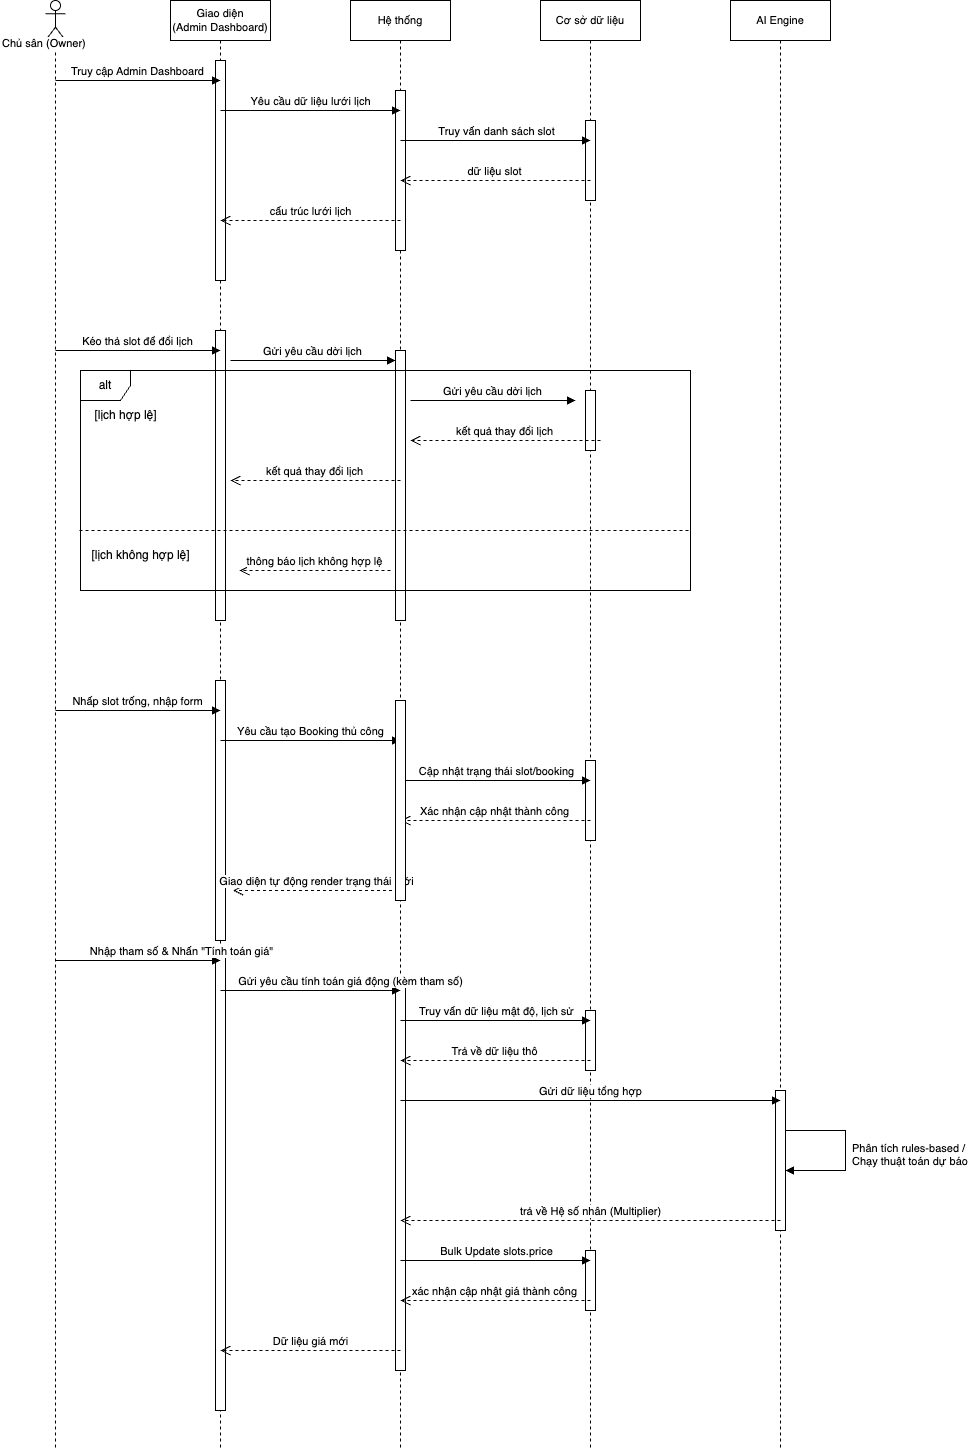
\includegraphics[width=0.95\textwidth]{Images/sq_quan_ly_lich_va_dinh_gia.png}
    \caption{Biểu đồ tuần tự luồng Quản lý lịch và định giá của Chủ sân}
    \label{fig:sequence_slot_management}
\end{figure}

\subsection{Đặc tả Use Case: Sử dụng mã QR để Check-in tại sân (B2C)}
\textbf{Tác nhân:} Người chơi \\
\textbf{Mục đích:} Hỗ trợ người chơi tự động xác nhận sự hiện diện tại quầy một cách nhanh chóng, không cần đối chiếu thủ công. \\
\textbf{Luồng sự kiện chính:}
\begin{enumerate}
    \item Người chơi mở ứng dụng và truy cập vào Đơn đặt sân.
    \item Hệ thống sinh ra và trả về một mã QR Token duy nhất cho đơn hàng.
    \item Người chơi tiến hành quét mã QR này tại thiết bị/quầy của sân.
    \item Mã QR Token được gửi về hệ thống để xác thực. Hệ thống kiểm tra tính hợp lệ của Booking.
    \begin{itemize}
        \item \textbf{Hợp lệ:} Hệ thống cập nhật trạng thái đơn hàng thành "Đã check-in" vào cơ sở dữ liệu và hiển thị thông báo thành công.
        \item \textbf{Không hợp lệ:} Hệ thống hiển thị lỗi "Mã QR không hợp lệ" trên giao diện.
    \end{itemize}
\end{enumerate}

\begin{figure}[H]
    \centering
    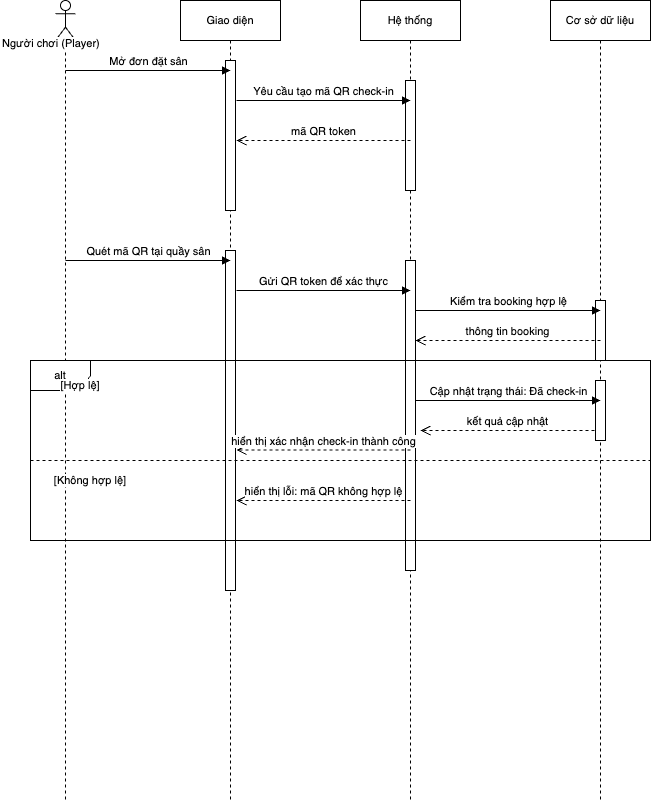
\includegraphics[width=0.95\textwidth]{Images/sq_checkin_qr.png}
    \caption{Biểu đồ tuần tự luồng Sử dụng mã QR để Check-in}
    \label{fig:sequence_checkin}
\end{figure}

\subsection{Đặc tả Use Case: Đánh giá chất lượng sân (B2C)}
\textbf{Tác nhân:} Người chơi \\
\textbf{Mục đích:} Thu thập phản hồi từ khách hàng sau khi trải nghiệm dịch vụ để xây dựng hệ thống xếp hạng uy tín cho các cụm sân. \\
\textbf{Luồng sự kiện chính:}
\begin{enumerate}
    \item Người chơi truy cập vào mục Lịch sử đặt sân.
    \item Hệ thống truy vấn cơ sở dữ liệu và trả về danh sách các Booking có trạng thái "Đã hoàn thành".
    \item Người chơi chọn một Booking cụ thể, nhập điểm số (Rating) và nội dung đánh giá (Review), sau đó nhấn Gửi.
    \item Hệ thống thực hiện Validate (kiểm tra tính hợp lệ) và lưu dữ liệu đánh giá mới.
    \item Hệ thống tự động tính toán lại và cập nhật Điểm trung bình của cụm sân tương ứng.
    \item Trả về thông báo "Đánh giá thành công" trên giao diện người chơi.
\end{enumerate}

\begin{figure}[H]
    \centering
    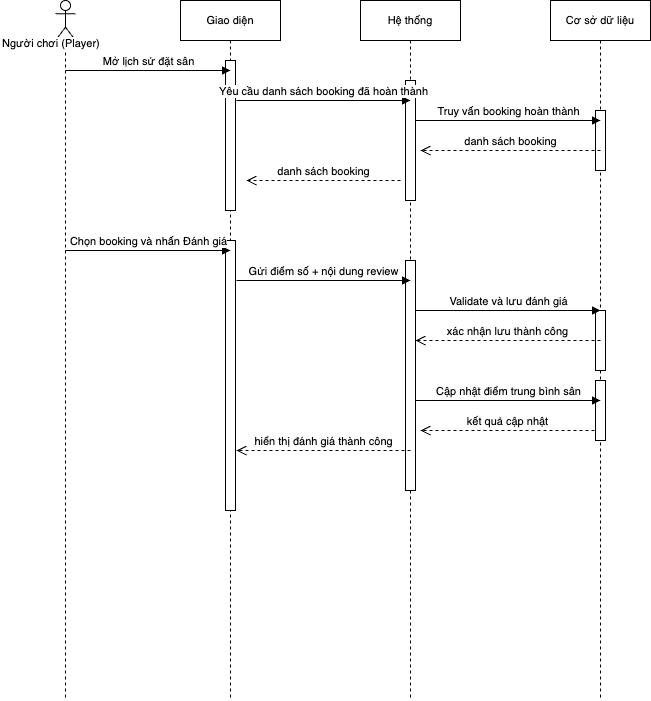
\includegraphics[width=0.95\textwidth]{Images/sq_danh_gia_san.png}
    \caption{Biểu đồ tuần tự luồng Đánh giá chất lượng sân}
    \label{fig:sequence_review}
\end{figure}

\subsection{Đặc tả Use Case: Tạo phòng và Tham gia ghép trận - Matchmaking (B2C)}
\textbf{Tác nhân:} Người chơi \\
\textbf{Mục đích:} Kết nối các cá nhân có cùng trình độ và nhu cầu thời gian để lập nhóm chơi chung, giúp san sẻ chi phí thuê sân. \\
\textbf{Luồng sự kiện chính:}
\begin{enumerate}
    \item Người chơi mở tính năng Ghép trận trên ứng dụng. Hệ thống truy vấn và hiển thị danh sách các phòng đang mở kèm theo thông tin trình độ.
    \item \textbf{Tạo phòng mới:} Người chơi chọn sân, khung giờ, thiết lập yêu cầu trình độ và gửi yêu cầu tạo phòng. Hệ thống lưu thông tin phòng mới, sinh mã phòng và trả về cho người dùng.
    \item \textbf{Tham gia phòng có sẵn:} Người chơi chọn một phòng trong danh sách và nhấn Tham gia. Hệ thống kiểm tra các slot còn trống trong phòng, tiến hành cập nhật trạng thái và trả về thông báo tham gia thành công.
\end{enumerate}

\begin{figure}[H]
    \centering
    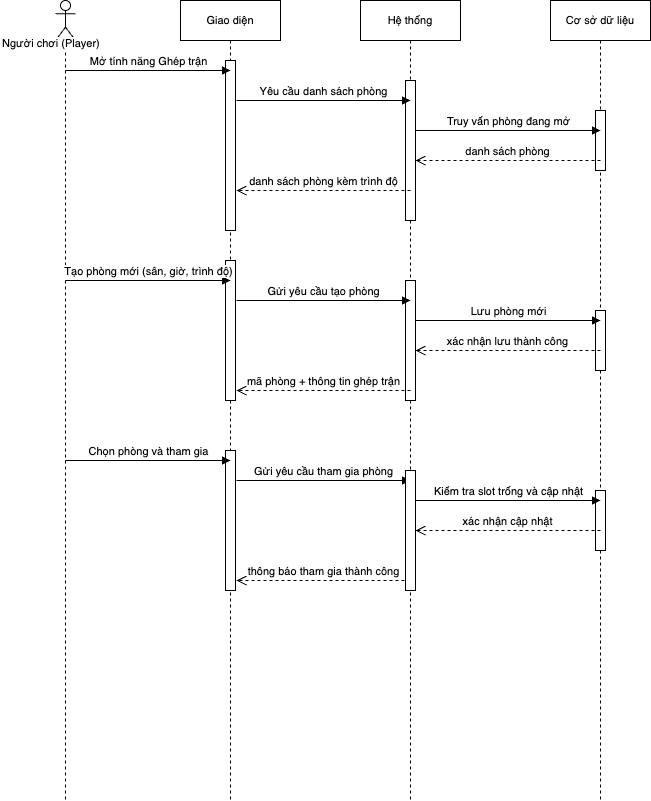
\includegraphics[width=0.95\textwidth]{Images/sq_ghep_tran.png}
    \caption{Biểu đồ tuần tự luồng Tạo phòng và Tham gia ghép trận}
    \label{fig:sequence_matchmaking}
\end{figure}

\subsection{Đặc tả Use Case: Quản lý danh mục sân (B2B)}
\textbf{Tác nhân:} Chủ sân \\
\textbf{Mục đích:} Cho phép chủ sân số hóa cơ sở vật chất, quản lý thông tin các cụm sân (Venue) và sân lẻ (Court) thuộc quyền sở hữu. \\
\textbf{Luồng sự kiện chính:}
\begin{enumerate}
    \item Chủ sân truy cập trang Quản lý danh mục trên Admin Dashboard. Hệ thống trả về danh sách Venue/Court hiện có.
    \item \textbf{Thêm sân:} Chủ sân nhập thông tin (tên, địa chỉ, tiện ích) và gửi yêu cầu. Hệ thống Validate và lưu sân mới vào DB.
    \item \textbf{Sửa thông tin:} Chủ sân chọn sân, cập nhật thông tin và nhấn Gửi. Hệ thống lưu thông tin mới.
    \item \textbf{Xóa sân:} Chủ sân chọn sân và xác nhận xóa. Hệ thống thực hiện lệnh Soft-delete (xóa mềm) trong DB để bảo toàn dữ liệu lịch sử đối soát và trả về kết quả thành công.
\end{enumerate}

\begin{figure}[H]
    \centering
    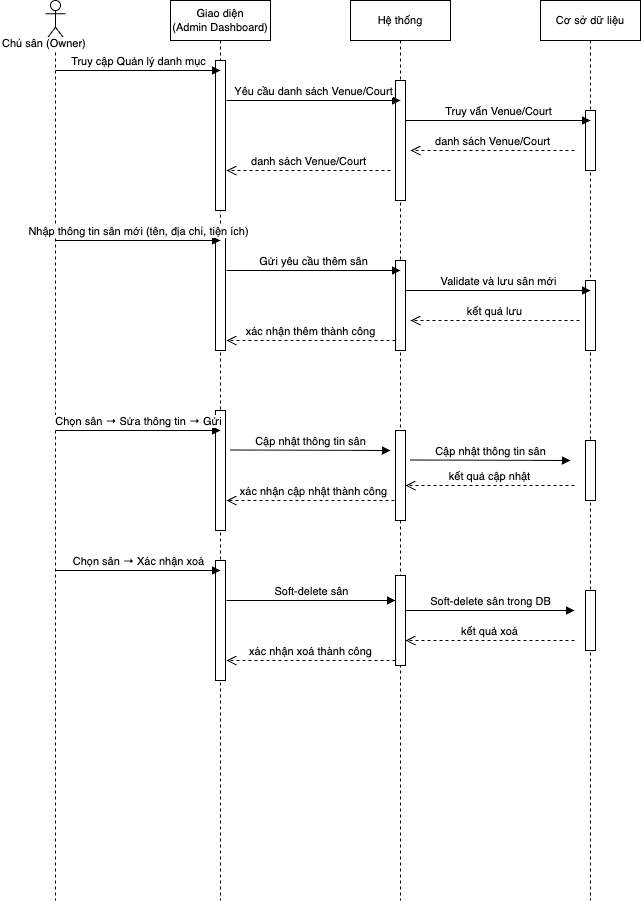
\includegraphics[width=0.95\textwidth]{Images/sq_quan_ly_danh_muc.png}
    \caption{Biểu đồ tuần tự luồng Quản lý danh mục sân}
    \label{fig:sequence_category}
\end{figure}

\subsection{Đặc tả Use Case: Đồng bộ Hóa đơn điện tử MISA (B2B)}
\textbf{Tác nhân:} Chủ sân \\
\textbf{Mục đích:} Tự động hóa quy trình xuất và đối soát hóa đơn điện tử cho các giao dịch đặt sân, đảm bảo tuân thủ pháp lý. \\
\textbf{Luồng sự kiện chính:}
\begin{enumerate}
    \item Chủ sân truy cập trang Hóa đơn. Hệ thống truy vấn và hiển thị danh sách các hóa đơn đã xuất hoặc chờ xử lý.
    \item Chủ sân chọn hóa đơn cần xử lý và nhấn "Đồng bộ MISA".
    \item Hệ thống CourtMate gọi API sang nền tảng MISA meInvoice để yêu cầu xuất hóa đơn.
    \item Sau khi nhận được kết quả từ MISA, hệ thống cập nhật trạng thái hóa đơn tương ứng trong cơ sở dữ liệu và hiển thị thông báo đồng bộ thành công cho Chủ sân.
\end{enumerate}

\begin{figure}[H]
    \centering
    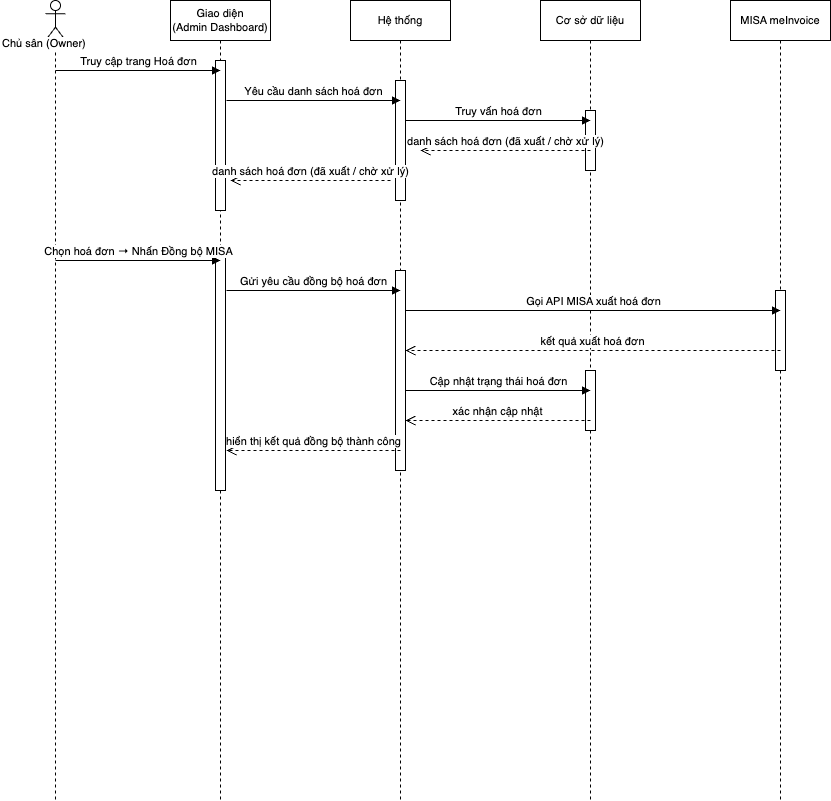
\includegraphics[width=0.95\textwidth]{Images/sq_quan_ly_hoa_don.png}
    \caption{Biểu đồ tuần tự luồng Đồng bộ Hóa đơn điện tử MISA}
    \label{fig:sequence_invoice}
\end{figure}

\subsection{Đặc tả Use Case: Cấu hình AI Định giá động và Xem báo cáo thống kê (B2B)}
\textbf{Tác nhân:} Chủ sân, AI Engine \\
\textbf{Mục đích:} Cung cấp bức tranh toàn cảnh về hiệu quả kinh doanh và cho phép chủ sân áp dụng AI để điều chỉnh giá tự động nhằm tối ưu lợi nhuận. \\
\textbf{Luồng sự kiện chính:}
\begin{enumerate}
    \item \textbf{Xem Báo cáo:} Chủ sân truy cập trang Thống kê. Hệ thống truy vấn và hiển thị Biểu đồ tài chính tổng quan. Khi chọn Biểu đồ nhiệt (Heatmap), hệ thống truy vấn mật độ slot để hiển thị công suất lấp đầy. Chủ sân có thể chọn khoảng thời gian để hệ thống tổng hợp và xuất file báo cáo (PDF/Excel).
    \item \textbf{Cấu hình AI Định giá:} Chủ sân nhập các tham số đầu vào và nhấn "Tính toán giá". Hệ thống tổng hợp dữ liệu (mật độ, lịch sử) và gửi sang AI Engine.
    \item AI Engine thực hiện phân tích rules-based hoặc chạy thuật toán dự báo để tính toán và trả về Hệ số nhân (Multiplier).
    \item Hệ thống thực hiện lệnh Bulk Update để cập nhật hàng loạt trường giá tiền (slots.price) trong cơ sở dữ liệu và tự động render dữ liệu giá mới lên giao diện cho Chủ sân.
\end{enumerate}

\begin{figure}[H]
    \centering
    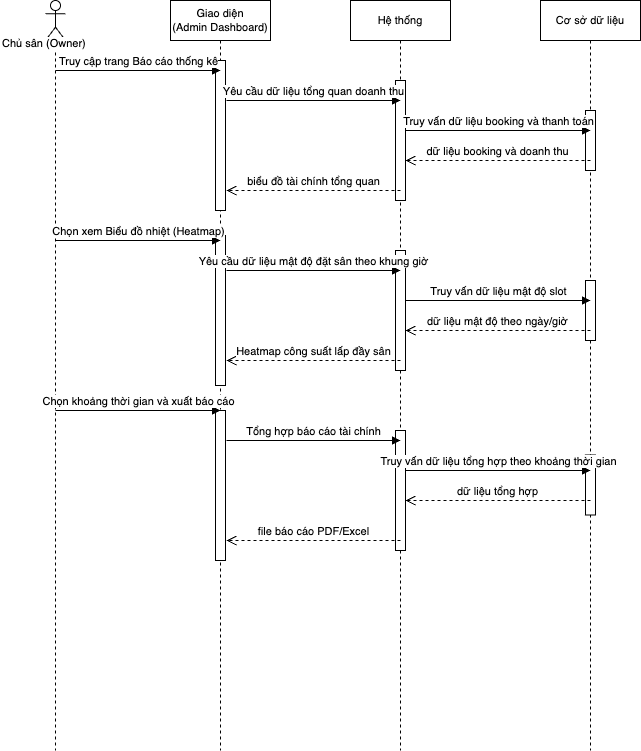
\includegraphics[width=0.95\textwidth]{Images/sq_bao_cao_thong_ke.png}
    \caption{Biểu đồ tuần tự luồng Cấu hình AI Định giá động và Xem báo cáo thống kê}
    \label{fig:sequence_report}
\end{figure}





\section{Kiến trúc hệ thống và Thiết kế kỹ thuật}

\subsection{Kiến trúc tổng thể (High-Level Architecture)}
Hệ thống CourtMate được xây dựng theo kiến trúc Pragmatic Microservices nhằm giải quyết bài toán xử lý lượng truy cập lớn (độ trễ dưới 10ms) nhưng vẫn cân bằng được chi phí vận hành ở giai đoạn sản phẩm tối thiểu (MVP).

\begin{figure}[H]
    \centering
    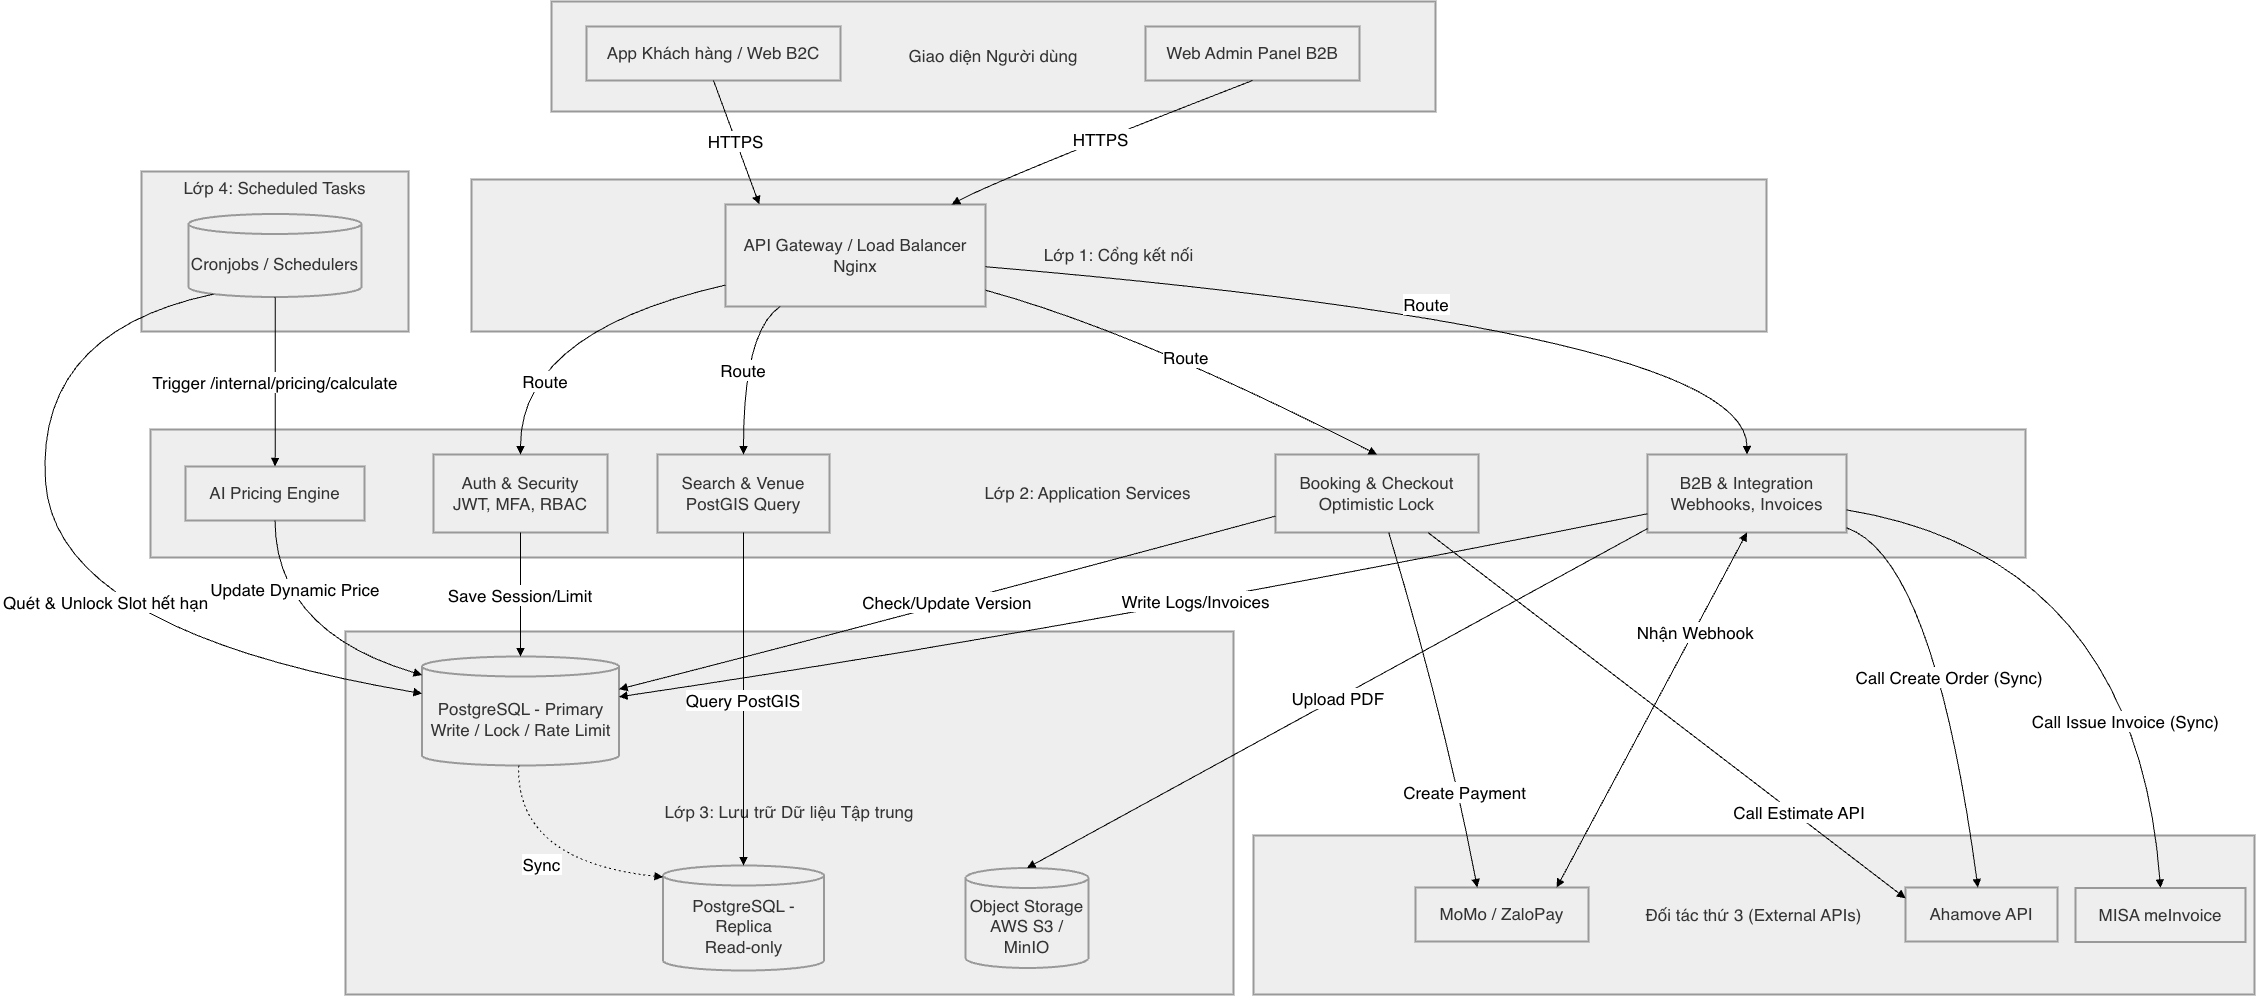
\includegraphics[width=1\textwidth]{Images/TMĐT_252-system.drawio.png}
    \caption{Sơ đồ kiến trúc hạ tầng tổng thể của hệ thống CourtMate}
    \label{fig:simplified_arch}
\end{figure}

Hình \ref{fig:simplified_arch} minh họa kiến trúc hạ tầng tổng thể của hệ thống CourtMate. Hệ thống được tổ chức thành các lớp (Layers) tách biệt nhằm đảm bảo tính linh hoạt và dễ quản lý. Kiến trúc này được lựa chọn nhằm ưu tiên tính khả thi, chi phí thấp và khả năng mở rộng tuyến tính cho giai đoạn MVP của hệ thống.

\subsection{Chi tiết các lớp kiến trúc phân tầng}

\subsubsection{Lớp Biên (Edge Layer - Lớp 1: Cổng kết nối)}
\begin{itemize}
    \item \textbf{Thành phần:} Nginx (đóng vai trò API Gateway và Load Balancer).
    \item \textbf{Nhiệm vụ:} Đây là điểm tiếp nhận duy nhất cho toàn bộ lưu lượng HTTPS từ App Khách hàng / Web B2C và Web Admin Panel B2B. Nginx chịu trách nhiệm phân giải (Routing) dựa trên đường dẫn URL để đưa request đến đúng cụm dịch vụ bên dưới một cách minh bạch.
\end{itemize}

\subsubsection{Lớp Ứng dụng (Application Layer - Lớp 2)}
Áp dụng chiến lược lập trình đa ngôn ngữ (Polyglot Programming), tách các module thành các service độc lập để dễ dàng mở rộng:
\begin{itemize}
    \item \textbf{Auth \& Security (JWT, MFA, RBAC):} Đứng trước các service nghiệp vụ để xác thực danh tính người dùng và phân quyền truy cập.
    \item \textbf{Search \& Venue (Node.js/Express):} Xử lý các truy vấn tìm kiếm sân bãi thông qua PostGIS, ưu tiên tốc độ I/O bất đồng bộ để đáp ứng lượng request khổng lồ.
    \item \textbf{Booking \& Checkout (Node.js/Express):} Xử lý luồng đặt sân hướng khách hàng, quản lý vòng đời đơn hàng và cơ chế giữ chỗ (Optimistic Lock).
    \item \textbf{B2B \& Integration (Java/Spring Boot 3.2):} Xử lý các tính năng quản trị phức tạp của chủ sân và giao tiếp đồng bộ (Sync) với các đối tác thứ ba (MISA meInvoice). Java Spring Boot đảm bảo tính chặt chẽ, toàn vẹn giao dịch (ACID).
    \item \textbf{AI Pricing Engine (Python/FastAPI):} Cô lập hoàn toàn logic tính toán Machine Learning nặng nề. Được kích hoạt bởi Cronjobs/Schedulers (Lớp 4), AI Engine sẽ tính toán giá mới và cập nhật thẳng xuống cơ sở dữ liệu mà không làm nghẽn luồng xử lý web chính.
\end{itemize}

\subsubsection{Lớp Dữ liệu (Data Layer - Lớp 3: Lưu trữ Dữ liệu Tập trung)}
Hệ thống áp dụng mẫu thiết kế Shared Database Pattern (Dùng chung cơ sở dữ liệu) được tối ưu hóa:
\begin{itemize}
    \item \textbf{PostgreSQL (Primary):} Xử lý các luồng thao tác Ghi (Write), Khóa (Lock), và Giới hạn tỷ lệ (Rate Limit).
    \item \textbf{PostgreSQL (Replica - Read-only):} Được đồng bộ hóa từ cụm Primary. Kết hợp với PostGIS để chuyên biệt hóa cho các truy vấn Đọc (Read) và tìm kiếm không gian địa lý, giúp giảm tải tối đa cho cơ sở dữ liệu chính.
    \item \textbf{Object Storage (AWS S3 / MinIO):} Lưu trữ tài nguyên phi cấu trúc, tệp tĩnh như hình ảnh, file hóa đơn PDF.
\end{itemize}

\subsubsection{Lớp Hạ tầng và Đối tác (Infrastructure \& External APIs)}
Hệ thống kết hợp sức mạnh của Multi-Cloud:
\begin{itemize}
    \item Máy chủ tính toán đặt tại Việt Nam (như Bizfly/Viettel Cloud) để đạt độ trễ mạng cực thấp.
    \item Tích hợp sâu vào các Webhook/API ngoại vi: VietQR (Dòng tiền tài chính), MISA (Hóa đơn điện tử).
\end{itemize}
